\chapter{Aplicação a dados de Montes Claros de Goiás}
\label{sec:real_application}

A província alcalina de Goiás (PAGO) é uma região na parte central do Brasil onde há ocorrências de magmatismos máficos-ultramáficos alcalinos. Esta região apresenta rochas com extensas variedades petrográficas. Ao longo desta área existem complexo máficos-ultramáficos (intrusões plutônicas), intrusões alcalinas sub-vulcânicas (diátremas) e produtos vulcânicos (lava kamafugítica) com diversos diques. Alguns dos principais complexos da PAGO são: Montes Claros de Goiás, Diorama, Córrego dos Bois, Morro do Macaco e Fazenda Buriti. Estas intrusões alcalinas são cercadas por um embasamento Pré-cambriano e rochas sedimentares do Fanerozóico da bacia do Paraná \citep{junqueira_brod_2005,carlson_etal_2007,marangoni_mantovani_2013,dutra_etal_2014}. Estudos recentes indicam que tais intrusões 
possuem intensa magnetização remanente \citep{marangoni_mantovani_2013,oliveirajr_etal_2015,marangoni_etal_2016,zhang_etal_2018}.

Esta região foi alvo de um levantamento aeromagnético com espaçamento entre as linhas norte-sul de $\sim 500$ m e de $\sim 8$ ao longo de cada linha, a uma altura constante de $100$ m acima do terreno. A direção do campo geomagnético para esta área era, respectivamente, de $-19.5^\circ$ e $-18.5^\circ$ para inclinação e declinação na época do levantamento. Invertemos os dados de anomalia de campo total para o complexo alcalino de Montes Claros de Goiás (Figura \ref{fig:data_fitting_real}a). Com o intuito de acelerar o processo de inversão, decimamos os dados ao longo da linha de voo, resultando em um grid de $55 \times 32$ pontos (um total de $N=1787$ observações). Esta nova configuração resulta em um espaçamento do grid de aproximadamente $300$ m e $500$ m ao longo dos eixos $x$ e $y$, respectivamente. Geramos uma camada equivalente composta por um grid de $55 \times 32$ dipolos (um total de $M=1787$ fontes equivalentes) posicionados a uma profundidade de $840$ m abaixo do plano de observação ($\sim 2$ vezes o maior espaçamento do grid). O algoritmo começa com uma aproximação inicial de $-70^\circ$ e $50^\circ$ para inclinação e declinação, respectivamente. A figura \ref{fig:data_fitting_real}b mostra os dados preditos produzidos pela camada equivalente. A figura \ref{fig:data_fitting_real}c mostra o mapa dos resíduos definido como a diferença entre os dados observados (Figura \ref{fig:data_fitting_real}a) e os dados preditos (Figura \ref{fig:data_fitting_real}b). Note que, dois locais na figura \ref{fig:data_fitting_real}c apresentam marcantes resíduos que, aparentemente, podem indicar a existência de fontes geológicas rasas. No entando, o histograma dos resíduos (Figura \ref{fig:data_fitting_real}d) é aceitável apresentando média de $-14.52$ nT (aproximadamente $0.1\% $ do valor máximo de anomalia de campo total) e desvio padrão de $312.28$ nT ($\sim 2 \% $ do valor máximo de anomalia de campo total). A direção de magnetização estimada $\bar{\mathbf{q}}$ tem inclinação $-50.2^\circ$ e declinação $34.9^\circ$. As figuras \ref{fig:dist_momentos_pos_real} e \ref{fig:convergence_real} mostram a distribuição de momentos magnéticos estimada $\bar{\mathbf{p}}$ e a convergência do algoritmo. Checamos a qualidade da direção de magnetização estimada calculando a redução ao polo da anomalia de campo total observada. Notamos que a anomalia reduzida ao polo (Figura \ref{fig:rtp_mc_data}) exibe valores predominantemente positivos e decai a zero quando se aproxima da borda da área de estudo. Por esta razão, consideramos que a direção de magnetização estimada leva a uma satisfatória anomalia reduzida ao polo. Concluimos com estes resultados que a distribuição de momentos magnéticos positiva e a direção de magnetização estimada produz um ajuste aceitável dos dados observados. A direção de magnetização estimada sugere também a existência de magnetização remanente para as intrusões na área de estudo.  

%% Figuras para aplicação a dados reais 
\begin{figure}
	\centering
	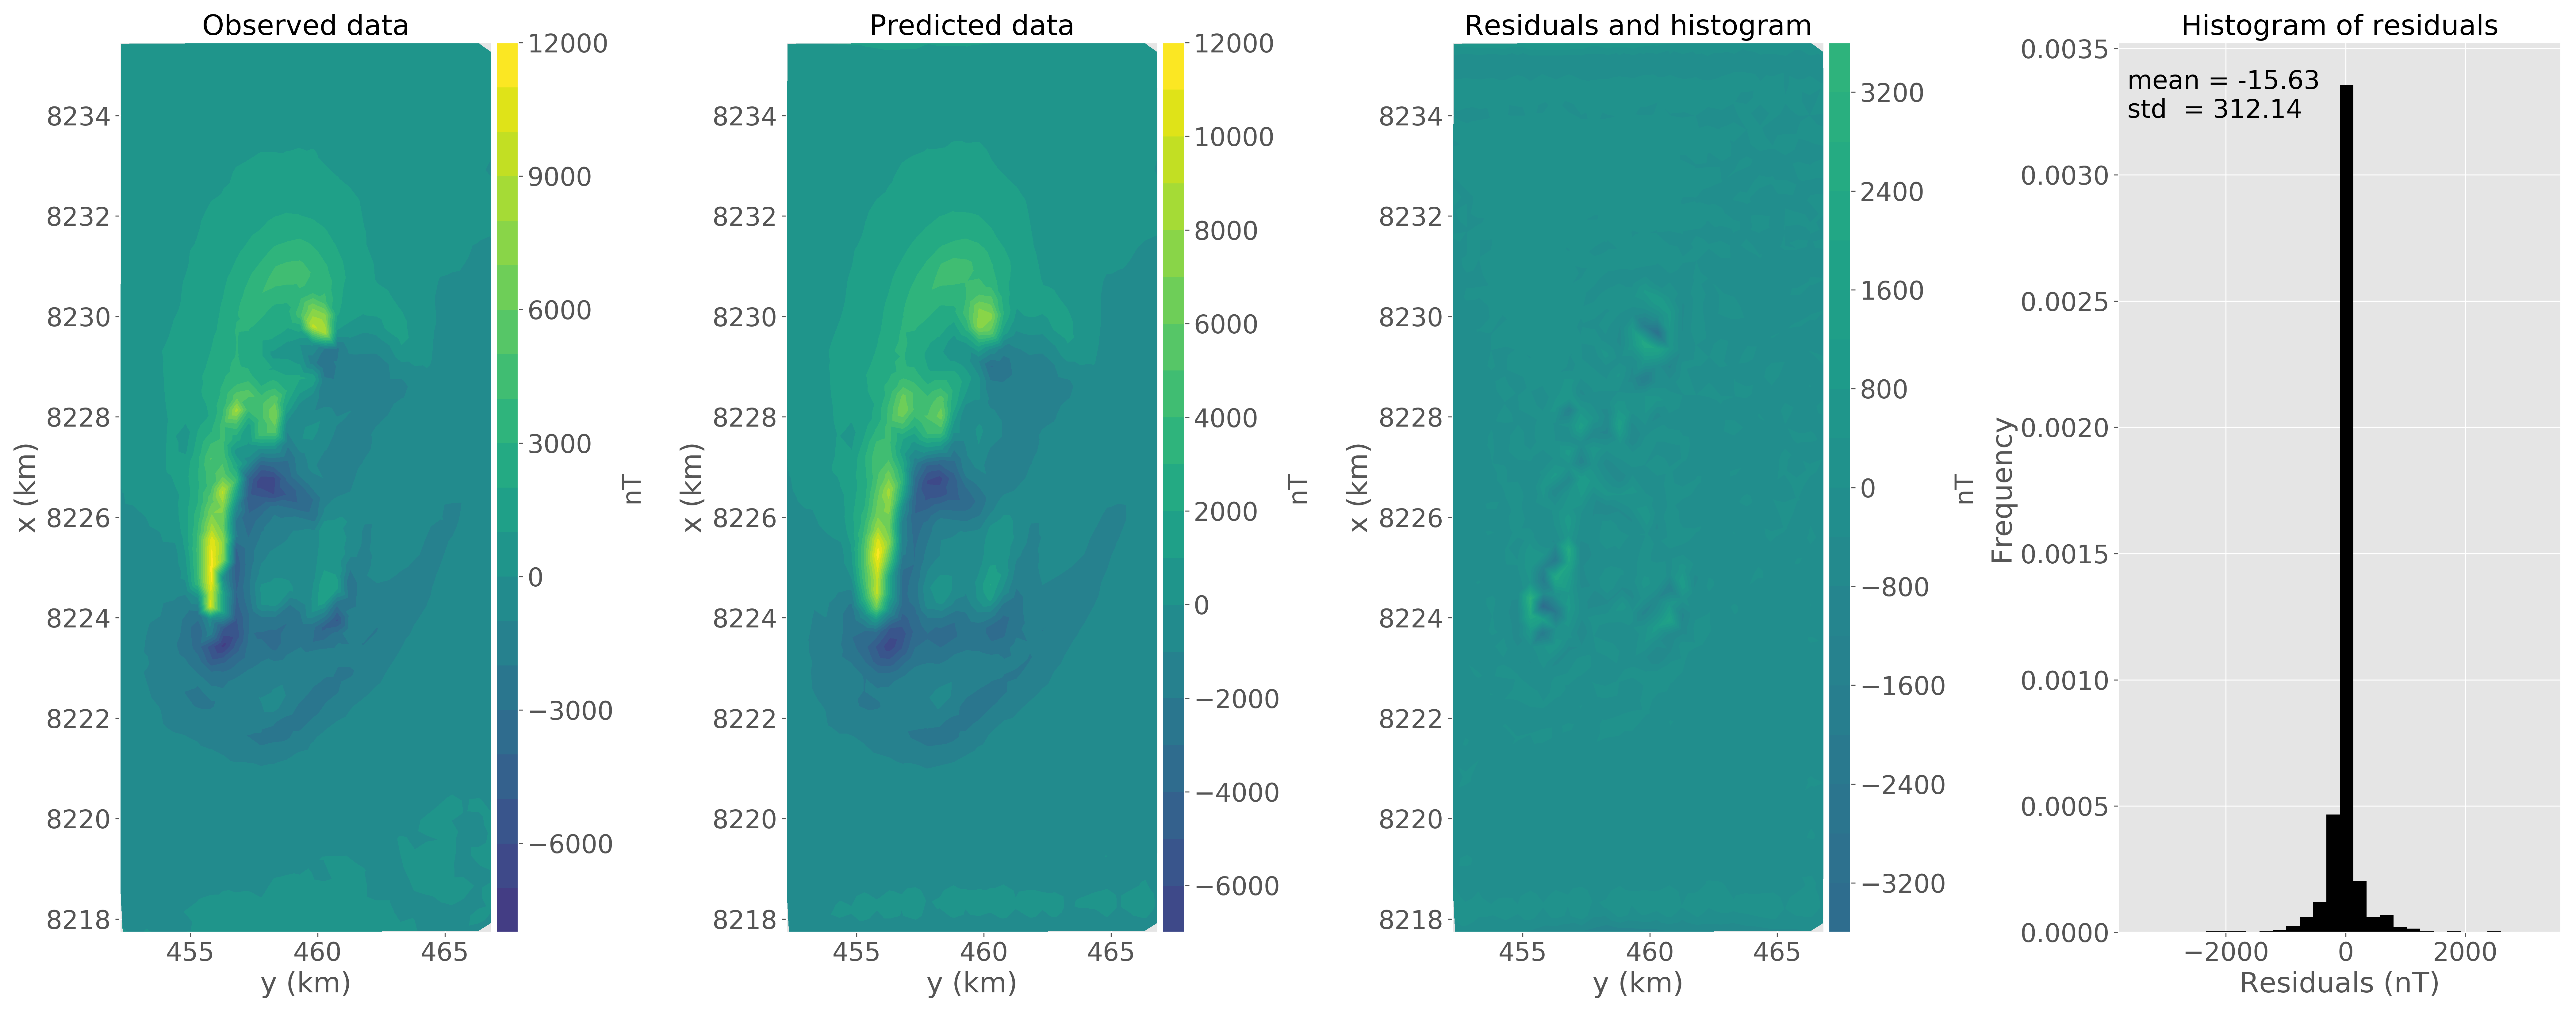
\includegraphics[width=1.1\textwidth]{Fig/eqlayer/field_data_montes_claros/data_fitting_LM_NNLS_montesclaros.png}
	\caption{Aplicação a dados reais para o complexo de Montes Claros de Goiás. (a) Anomalia de campo total observada. (b) Dados preditos produzido pela camada equivalente. (c) Diferença entre os dados mostrados nos gráficos a e b. (d) Histograma dos resíduos.}
	\label{fig:data_fitting_real}
\end{figure}

\begin{figure}
	\centering
	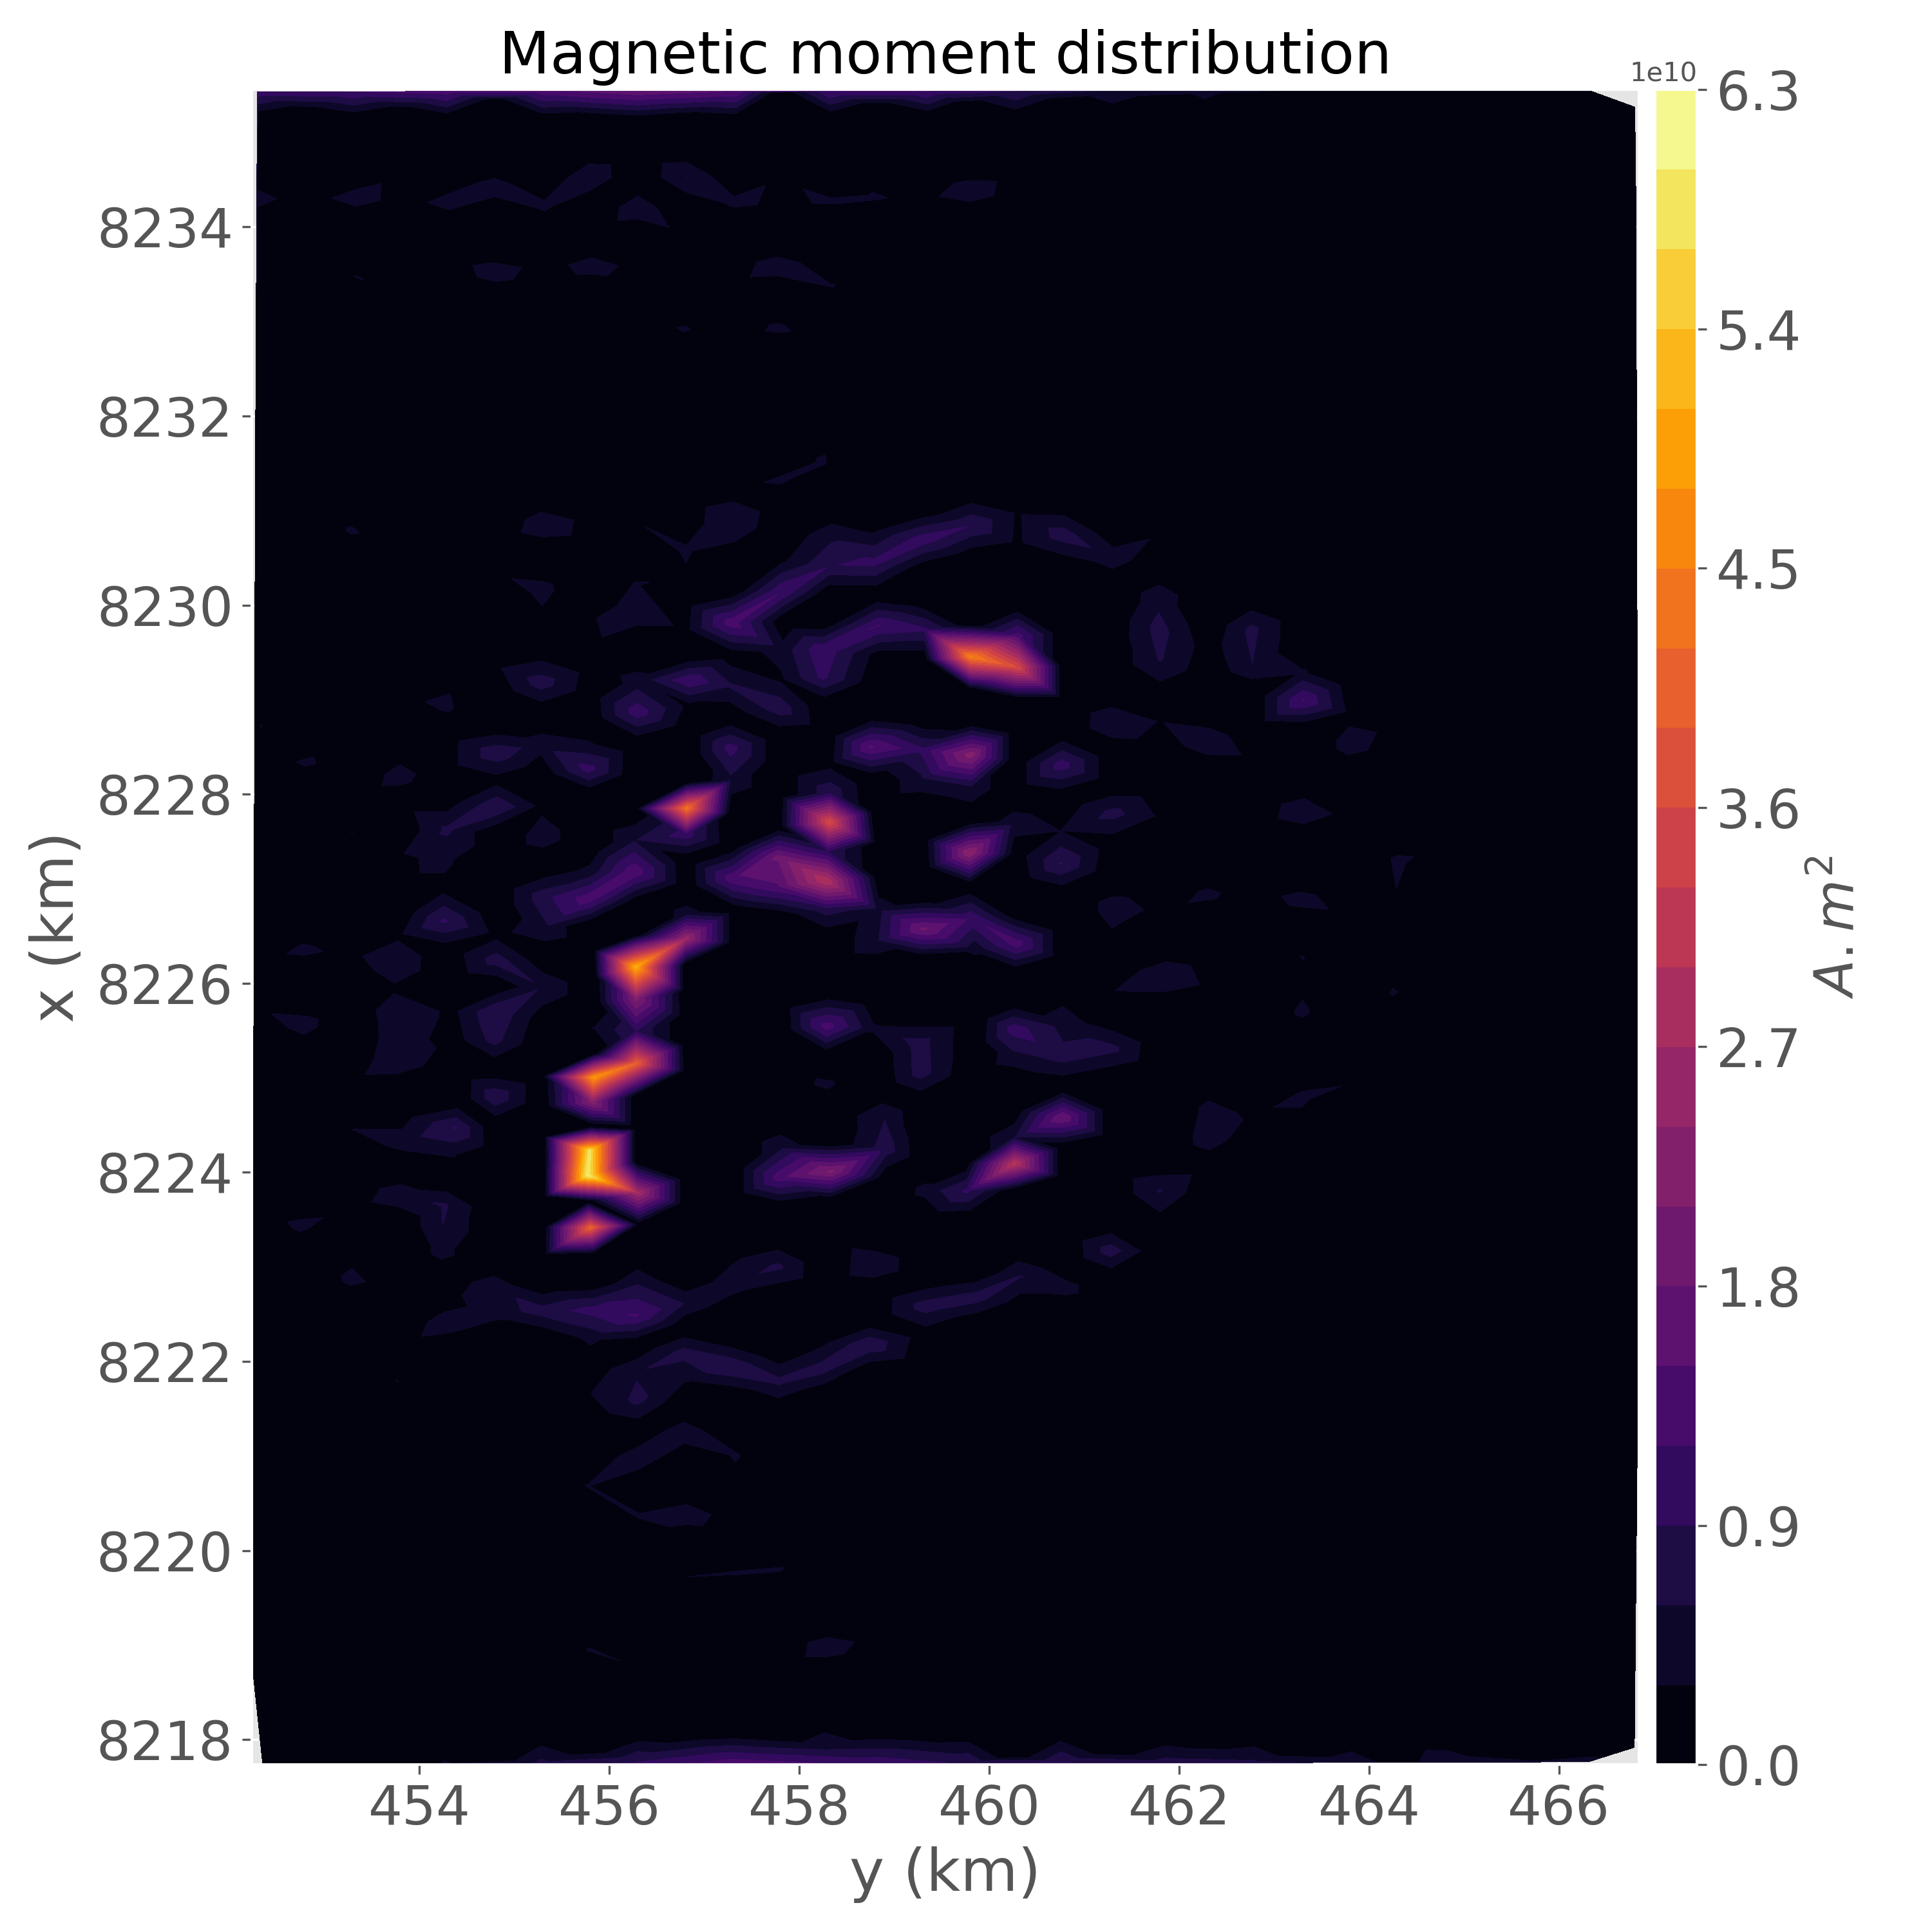
\includegraphics[width=.9\textwidth]{Fig/eqlayer/field_data_montes_claros/magnetic_moment_positive_LM_NNLS_montesclaros.png}
	\caption{Distribuição de momentos magnéticos positiva para a aplicação a dados reais no complexo de Montes Claros de Goiás.}
	\label{fig:dist_momentos_pos_real}
\end{figure}

\begin{figure}
	\centering
	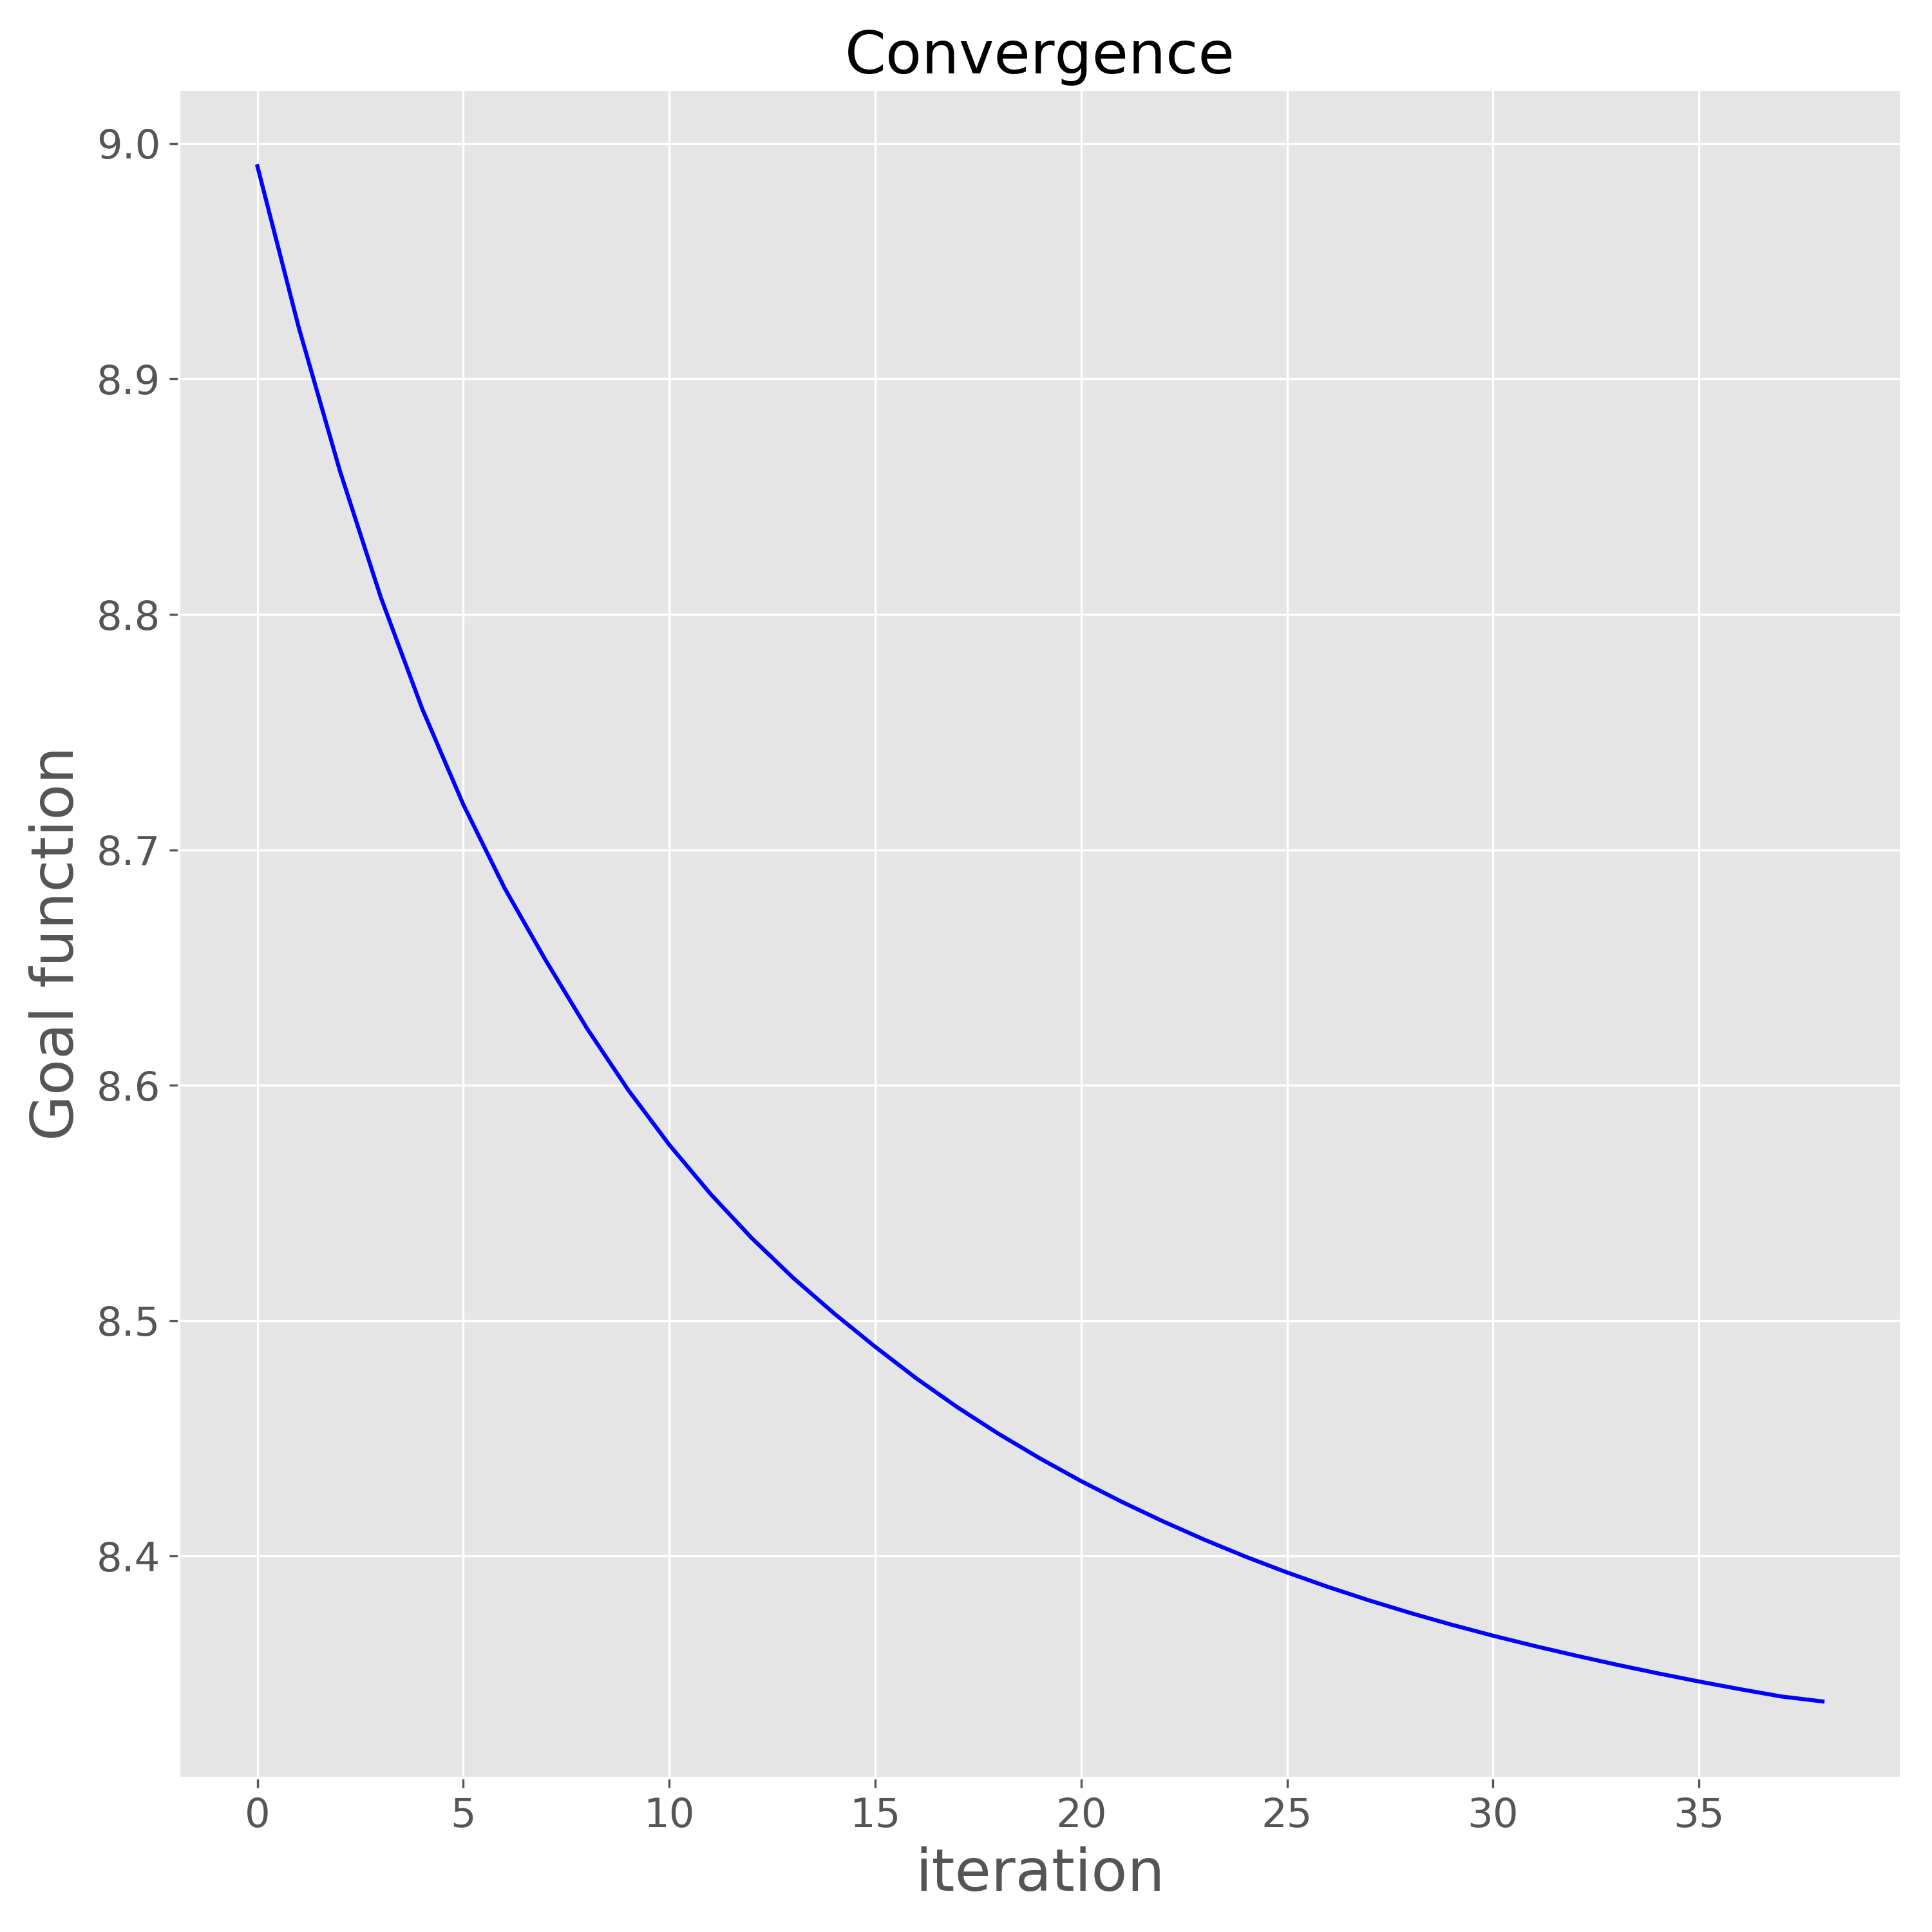
\includegraphics[width=.9\textwidth]{Fig/eqlayer/field_data_montes_claros/convergence_LM_NNLS_montesclaros.png}
	\caption{Valor da função objetivo ao longo das iterações (equação \ref{eq:positivity_goal_function}a) mostrando a convergência do algoritmo.}
	\label{fig:convergence_real}
\end{figure}

\begin{figure}
	\centering
	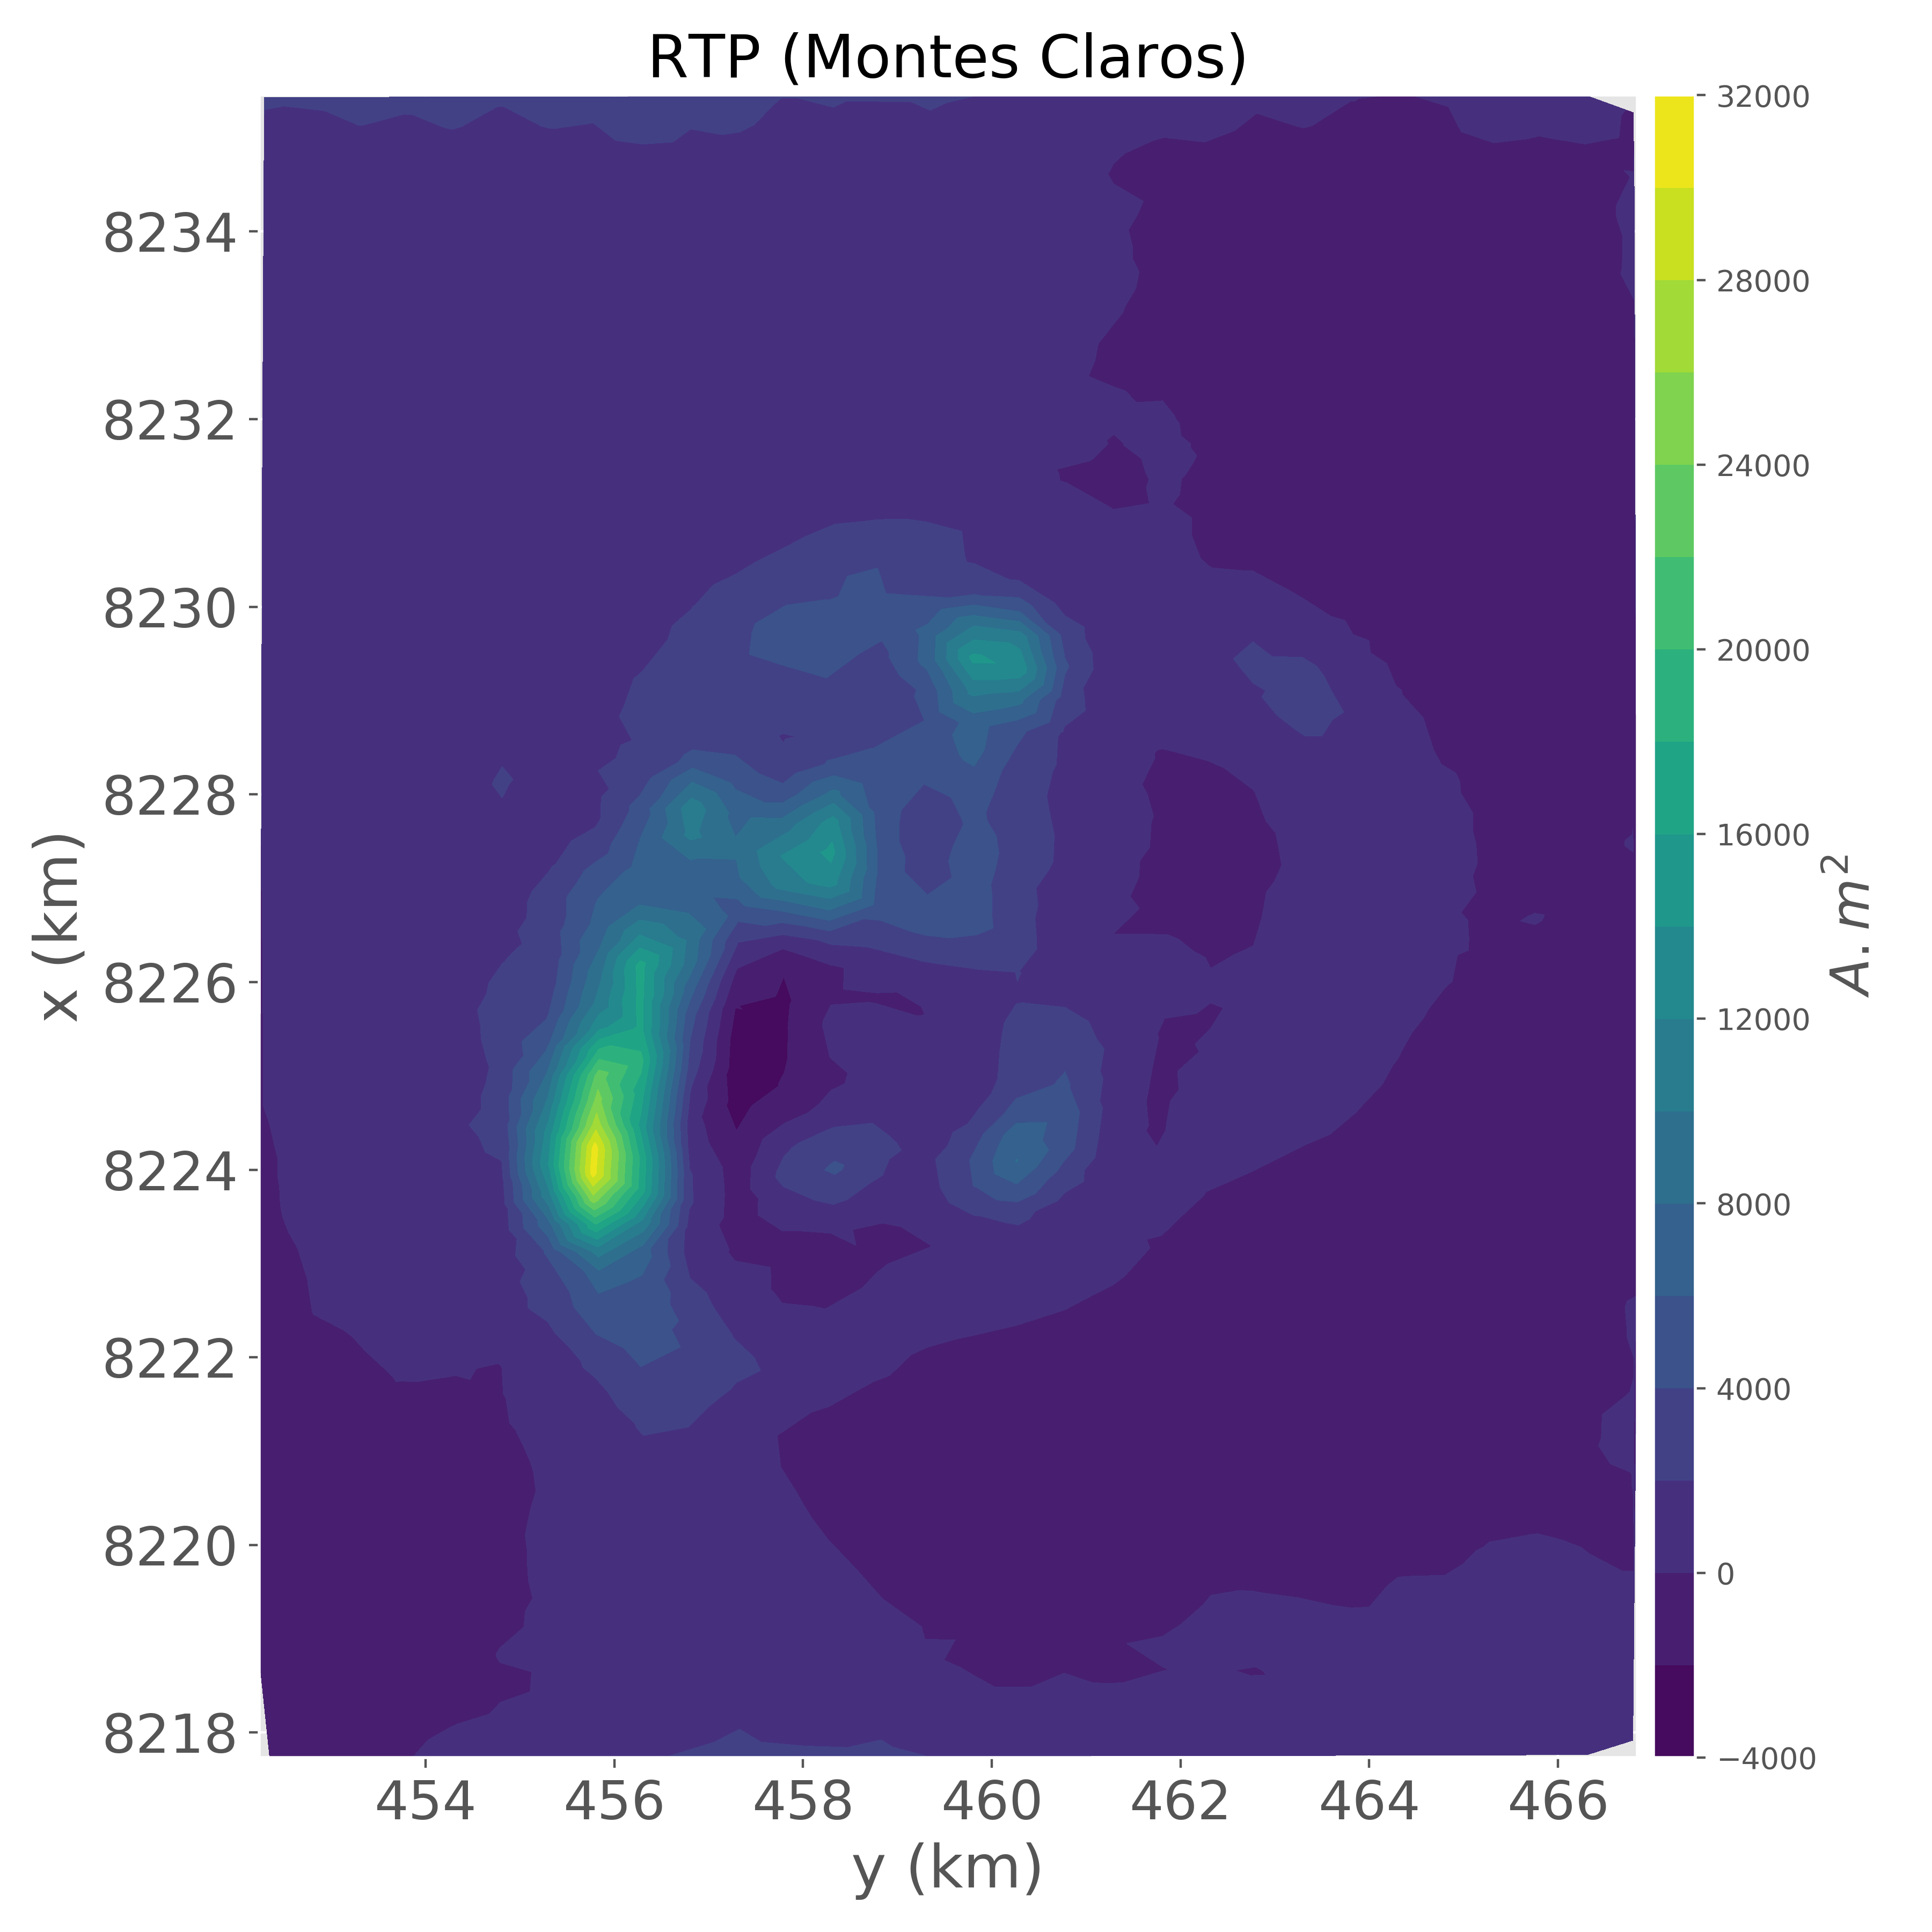
\includegraphics[width=.9\textwidth]{Fig/eqlayer/field_data_montes_claros/RTP_data_montes_claros.png}
	\caption{Redução ao polo dos dados reais do complexo de Montes Claros de Goiás (Figura \ref{fig:data_fitting_real}a) utilizando a 
	distribuição de intensidades de momentos magnéticos estimada mostrada na Figura \ref{fig:dist_momentos_pos_real}}
	\label{fig:rtp_mc_data}
\end{figure}

